%%% tech_notes.tex --- Technical notes about multitask sfan.

\documentclass[12pt,a4paper]{article}
\usepackage[T1]{fontenc}     
\usepackage[utf8]{inputenc}            % Accents codés dans la fonte
% \usepackage[frenchb]{babel}            % Les traductions françaises

\usepackage[runin]{abstract}           % Section "Résumé"
\usepackage{amssymb}                   % Symboles mathématiques
\usepackage{amsmath}                   % Plus de symboles mathématiques
\usepackage{amsthm}                    % Theorems
\usepackage{enumitem}                  % Personalisation des listes
\usepackage[margin=2cm]{geometry}      % Gestion des dimensions des pages
\usepackage{graphicx}                  % Gestion des inclusions graphiques
\usepackage{hyperref}                  % Inclusion d'URLs et de liens hypertexte
\usepackage[svgnames]{xcolor}          % Pour la gestion des couleurs

% Hyperref
% for a list of colors: p38 of http://mirrors.ibiblio.org/CTAN/macros/latex/contrib/xcolor/xcolor.pdf
\hypersetup{colorlinks=true,    % false: boxed links; true: colored links
            linkcolor=teal,     % color of internal links
            citecolor=teal}     % color of links to bibliography
% Font
%\usepackage[bitstream-charter]{mathdesign}
\usepackage[charter]{mathdesign}
%\usepackage{arev}



% Mathematical notations
\newtheorem{thm}{Theorem}

%\newcommand{\sset}{\mathcal{S}}
\newcommand{\sset}{S}
%\newcommand{\vset}{\mathcal{V}}
\newcommand{\vset}{V}
\DeclareMathOperator*{\argmax}{arg\,max}
\DeclareMathOperator*{\argmin}{arg\,min}


\newcommand{\caz}[1]{{\color{purple}[TODO (CA) : #1]}}


\title{Multitask selection of features as nodes}
\author{Chloé-Agathe Azencott}
\date{March 2016}

\begin{document}

\maketitle


\section{Introduction}
% L'analyse de données génome entier dans le but de déterminer quelles régions du génome sont associées à un phénotype particulier sont souvent limitées par la faiblesse du nombre d'échantillons étudiés devant celui de variables mesurées. Ce phénomène statistique est particulièrement amplifié dans le cas des études type GWAS (Genome-Wide Association Studies), dans lesquelles les variables mesurées sont des mutations d'une paire de bases (Single Nucleotide Polymorphisms, ou SNPs) au nombre de plusieurs centaines de milliers. \\

% On parlera ainsi dans la suite de SNPs mais il pourrait tout aussi bien s'agir d'autres variables génomiques (expression de gène, méthylation, etc).\\

% Traditionnellement, ces études utilisent un test statistique pour évaluer l'association entre chaque SNP et le phénotype étudié, indépendamment les uns des autres. Elles ne prennent ainsi aucunement en compte la possibilité d'une interaction entre ces SNPs. Cependant, même un modèle linéaire (qui ne suppose donc que des effets additifs) souffre de ce problème de grande dimensionalité. En effet, une régression linéaire cherchant à expliquer le phénotype $y$ comme une combinaison linéaire $\sum_{j=1}^p w_j x_j$ des $p$ SNPs résultera en un système sous-déterminé : il n'y a pas de solution unique pour les poids $\{w_j\}_{j=1, \dots, p}$. \\

% Afin de restreindre le nombre de solutions possible, il est fréquent dans ce cas d'imposer des contraintes sur l'espace des solutions. On parle alors de régularisation. C'est par exemple ce que fait l'approche du Lasso (Least absolute shrinkage and selection operator)~\cite{tibshirani96}, qui impose de mettre un grand nombre de coefficients à zéro. On parle alors de {\it parcimonie} (ou \og sparsité \fg, de l'anglais {\it sparsity}). Le Lasso est une méthode de {\it sélection de variables} ({\it feature selection} en anglais), au sens où seules les variables ayant un coefficient non-nul sont sélectionnées pour être utilisées dans le modèle final.

\section{Related Work}
\subsection{SConES}
% Plus récemment, des travaux ont émergé pour imposer des contraintes supplémentaires, et en particulier pour forcer les variables sélectionnées à respecter une structure de réseau pré-définie. En particulier, nous avons proposé en 2013 une approche appelée SConES (Selecting Connected Explanatory SNPs)~\cite{azencott13} qui permette de sélectionner des SNPs qui soient (1) associés au phénotype ; (2) peu nombreux ; (3) connectés sur un réseau biologique donné. 

\paragraph{Formulation}
Given
\begin{itemize}
\item a set $\vset$ of variables, of size $p$ ($\vset = \{1, \dots, p\}$);  
\item $\lambda, \eta \in \mathbb{R}^+$ two hyperparameters;
\item a network over $p$ nodes, corresponding to the $p$ variables, represented by its adjacency matrix $W$;
% \item $X \in \{0, 1, 2\}^{n \times p}$ le génotype de ces $p$ SNPs pour $n$ échantillons (chaque SNP est représenté par le nombre d'allèles mineurs) ;
\item $c \in \mathbb{R}^p$ the importance of each variable with respect to the task of interest,
% \item $y \in \mathbb{R}^n$ le phénotype de ces $n$ échantillons,
\end{itemize}

% On cherche ensuite à trouver le sous-ensembles $\sset$ de $\vset$ tel que : 
we want to find the subset $\sset$ of $\vset$ such that:
\begin{equation}
\argmax_{\sset \subseteq \vset }  \sum_{i \in \sset} c_i - \eta |\sset|
- \lambda \sum_{i \in \sset} \sum_{j \notin \sset} W_{ij} 
\label{eq:scones}
\end{equation}

The importance $c_1, \dots, c_p$ can be given by Pearson's correlation between data $X$ and outcome $y$.
In the case of SNP data, we can use a statistical test such as Linear SKAT~\cite{wu11}.

$\sset$ maximizes the sum of three terms:
\begin{enumerate}
\item The importance $\sum_{i \in \sset} c_i$ of $\sset$ for the task at hand;
\item A sparsity term $- \eta |\sset|$, which grows when the number of selected variables ($|\sset|$) is low;
\item A connectivity term $- \lambda \sum_{i \in \sset} \sum_{j \notin \sset} W_{ij} $, which is large when there are few links in the network connecting a selected variable to one that is not selected.
\end{enumerate}

Hyperparameters $\lambda$ and $\eta$ control the relative importance of each regularization term.

\paragraph{Solution}
This formulation is equivalent to a minimum $s/t$ cut problem on a network that can be built from the data and is presented on Figure~\ref{fig:mincut_scones}. The problem can then efficiently be solved with well-established maximum flow algorithms.\\

A detailed proof of the equivalence is available in~\cite{azencott13}. 

\begin{figure}[h]
  \centering
  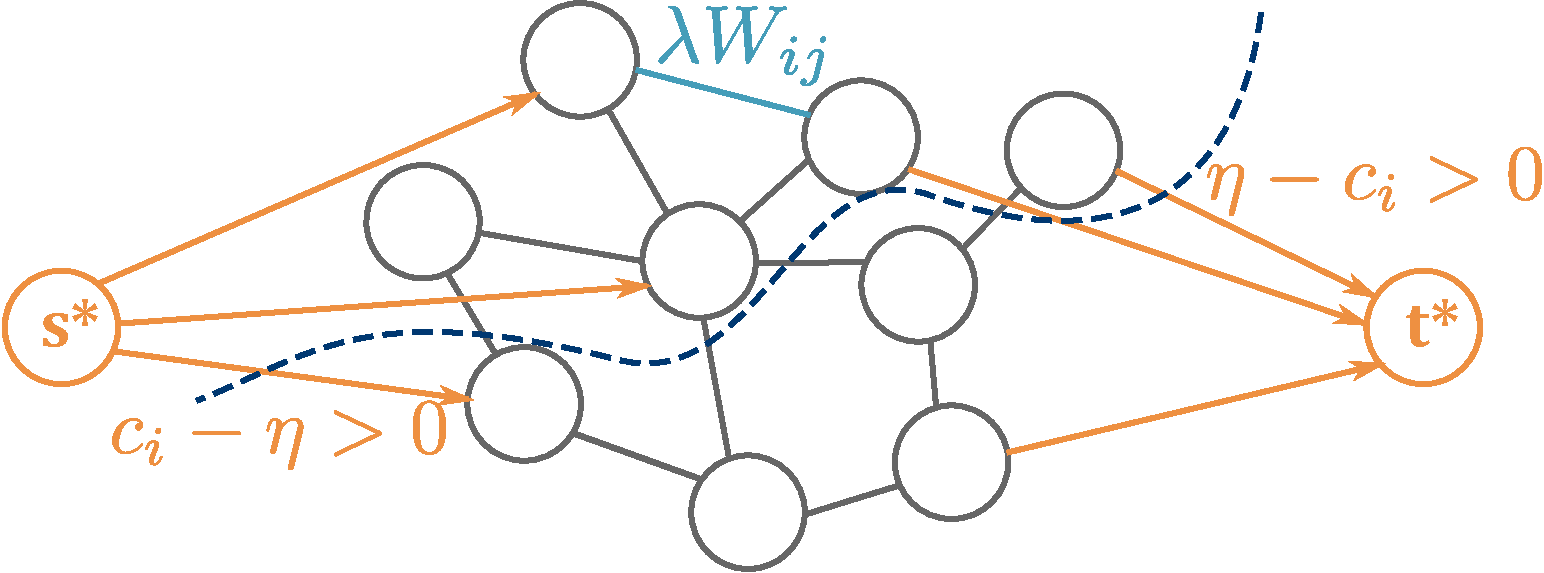
\includegraphics[width=0.5\textwidth]{figures/mincut_scones}
  \caption{Finding the minimum cut of this network is equivalent to solving the SConES optimization problem defined by ~\ref{eq:scones}.}
  \label{fig:mincut_scones}
\end{figure}



\subsection{MultiSConES}
% Une autre façon de réduire l'écart entre le nombre de variables et le nombre d'échantillons est d'augmenter le nombre d'échantillons. Cela peut être fait \og virtuellement \fg~si l'on dispose d'échantillons (les mêmes ou d'autres) pour lesquels d'autres phénotypes proches de celui qui nous intéresse ont été mesurés. Dans ce cas, on cherche à résoudre tous les problèmes de sélection de variable (correspondant à chaque phénotype) simultanément. C'est ce qu'on appelle une approche multi-tâches.\\

% Nous avons proposé en 2014 une extension multi-tâches de SConES, MultiSConES~\cite{sugiyama14}. Dans ce travail, on maximise une fonction qui comporte deux termes : 
% \begin{enumerate}
% \item La somme, pour les $K$ tâches, de la fonction optimisée pour SConES (Eq.~\ref{eq:scones}) ;
% \item Un terme $\mu \sum_{k=2}^K |\sset_{k-1} ~\Delta~ \sset_{k}| $ qui contrôle la différence symmétrique entre les ensembles de variables sélectionnées pour les différentes tâches.
% \end{enumerate}

% Cette nouvelle formulation peut aussi se résoudre par une reformulation mincut/maxflow.

\paragraph{Formulation}
\begin{equation}
\argmax_{\sset_1, \dots, \sset_K \subseteq \vset }  \sum_{k=1}^K \left (
\sum_{i \in \sset_k} c_i^k - \eta |\sset_k| - 
\lambda \sum_{i \in \sset_k} \sum_{j \notin \sset_k} W_{ij}^k \right ) - 
\mu  \sum_{k=1}^K \sum_{l > k} |\sset_{k} ~\Delta~ \sset_{l}|
\label{eq:multi_scones}
\end{equation}


\paragraph{Solution} 
This formulation is equivalent to finding a minimum $s/t$ cut on the super-network defined by connecting together the $K$ networks ($W^1, \dots, W^K$) as follows.

We define one node per (feature, task) pair.
\begin{itemize}
\item Node $(i, k)$ is connected to node $(i, l)$ 
  by an edge of weight $\mu$ (same feature, different task). 
\item Node $(i, k)$ is connected to node $(j, k)$
  by an edge of weight $\lambda W_{ij}^{k}$ (same task, different feature). 
\end{itemize}

We then add to the super-network two new nodes, a source $s^*$ and a sink $t^*$, 
which we connect to each node $(i, k)$ as follows:
\begin{itemize}
\item If $c_i^k - \eta \geq 0$, then we create an (oriented) edge from $s^*$ towards $(i, k)$,
  of weight $c_i^k - \eta$.
\item Else, we create an (oriented) edge from $(i, k)$ towards $t^*$, of weight $- (c_i^k - \eta)$.
\end{itemize}

This process is illustrated on Figure~\ref{fig:mincut_multiscones}.\\

\begin{figure}[h]
  \centering
  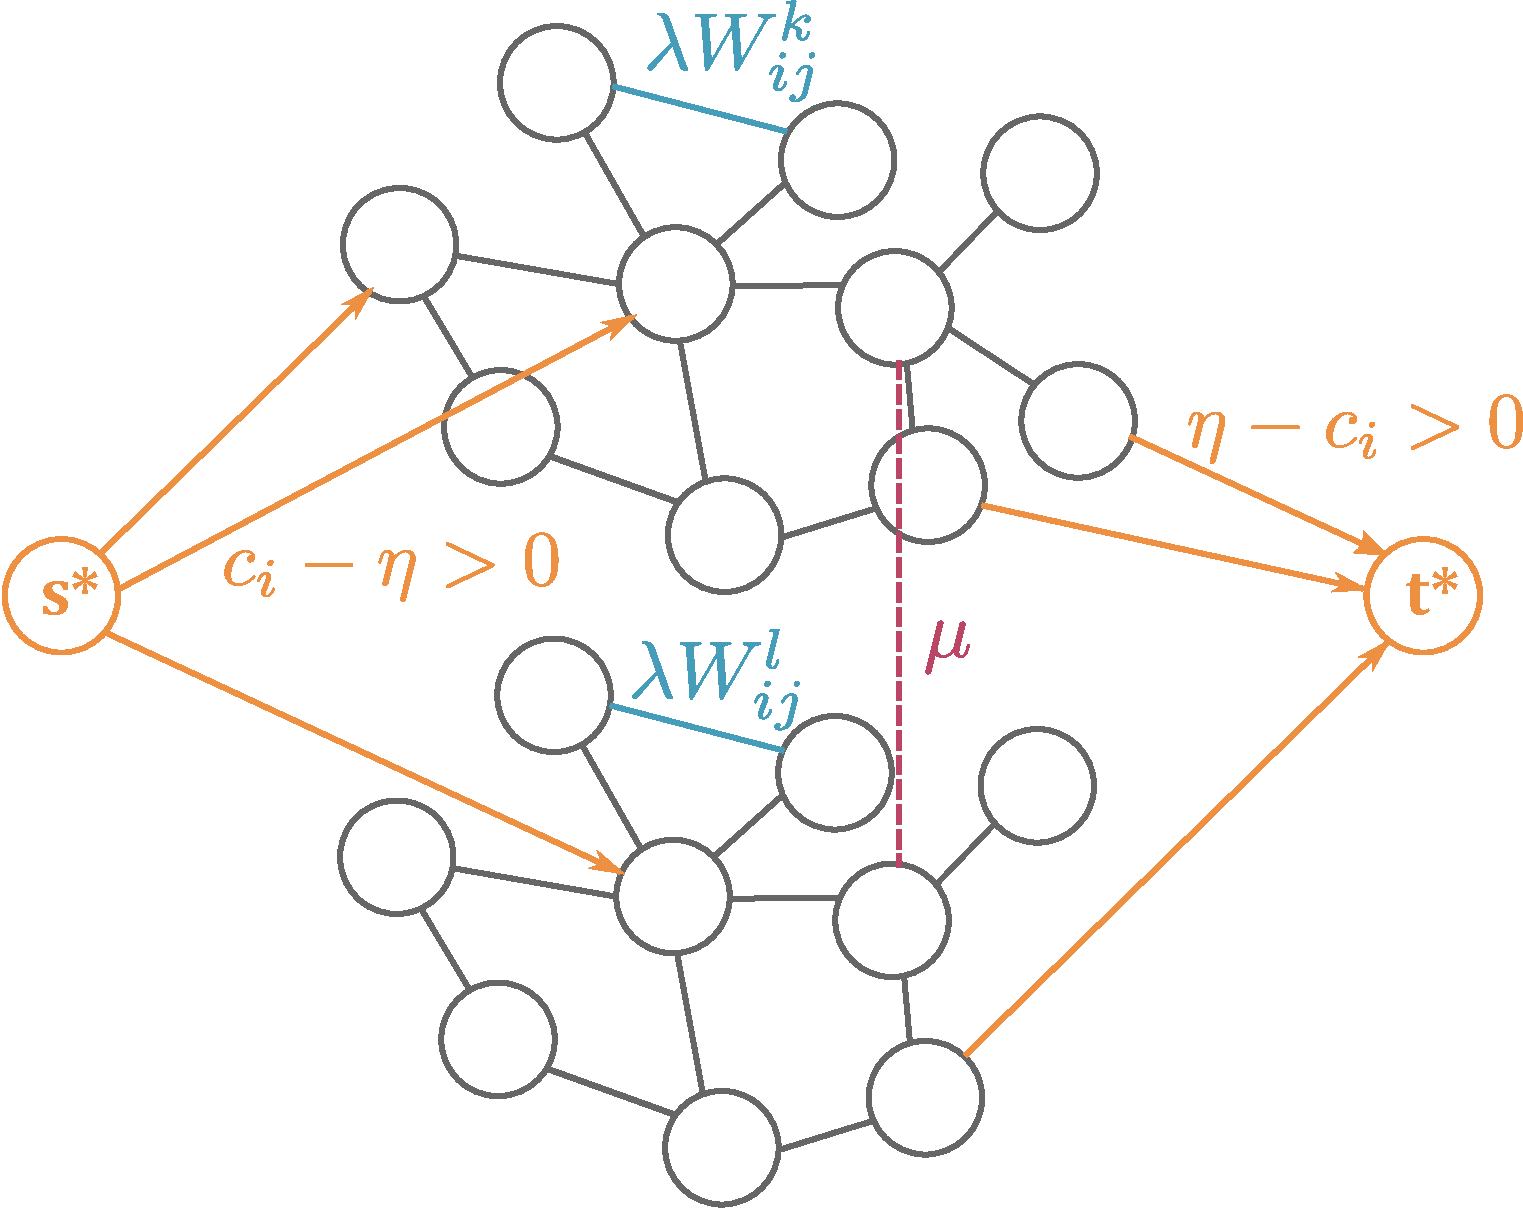
\includegraphics[width=0.5\textwidth]{figures/mincut_multiscones}
  \caption{Finding the minimum cut of this network is equivalent to solving the SConES optimization problem defined by ~\ref{eq:multi_scones}.}
  \label{fig:mincut_multiscones}
\end{figure}

\begin{thm}
  Finding a minimum $s/t$ cut on the super-network defined on Figure~\ref{fig:mincut_multiscones} is equivalent to solving Eq.~\ref{eq:multi_scones}.
\end{thm}


\begin{proof}
  The adjacency matrix $A$ of this network is defined by:
  \[
  A_{uv} =
  \begin{cases}
    - (c_i - \eta) & \mbox{ if } u = (i, k) \mbox{ and } v = t^{*} \\
    (c_i - \eta) & \mbox{ if } u = s^{*} \mbox{ and }  v = (i, k)\\
    \lambda W_{ij}^k & \mbox{ if } u = (i, k) \mbox{ and }  v = (j, k) \\
    \mu & \mbox{ if } u = (i, k) \mbox{ and } v = (i, l).
  \end{cases}
  \]

  Finding the minimum $s/t$ cut on a network defined by its adjacency matrix
  $A$ is equivalent to solving
  \[
  \argmin_{\sset \subseteq \vset} \sum_{u \in \sset} \sum_{v \notin \sset}
  A_{uv}.
  \]

  Hence finding the minimum $s/t$ cut on $A$ is equivalent to solving
  \[
  \argmin_{\sset_1, \ldots, \sset_K \subseteq \vset} \sum_{k=1}^K \left (
    \sum_{i \notin \sset_k, c_i^k \geq \eta} (c_i^k - \eta) + \sum_{i \in
      \sset_k, c_i^k < \eta} - (c_i^k - \eta) + \sum_{i \in \sset_k} \sum_{j
      \notin \sset_k} \lambda W_{ij}^k \right ) + \sum_{k=1}^K \sum_{l=1}^K
  \sum_{i \in \sset_k, i \notin \sset_l} \mu.
  \]

  Noting that
  \[ \sum_{i \notin \sset_k, c_i^k \geq \eta} (c_i^k - \eta) = \sum_{i, c_i^k
    \geq \eta} (c_i^k - \eta) - \sum_{i \in \sset_k, c_i^k \geq \eta} (c_i^k -
  \eta),\]

  that $\sum_{i, c_i^k \geq \eta} (c_i^k - \eta)$ is constant with respect to
  $\sset_1, \ldots, \sset_K$,

  and that
  \[
  \sum_{k=1}^K \sum_{l=1}^K \left( \sum_{i \in \sset_k, i \notin \sset_l} \mu
  \right) = \sum_{k=1}^K \sum_{l=1}^K \left( \sum_{i \in \sset_k \setminus
      \sset_l} \mu \right) = \mu \sum_{k=1}^K \sum_{l>k} |\sset_{k} ~\Delta~
  \sset_{l}|,
  \]


  the mincut problem is equivalent to:
  \[
  \argmin_{\sset_1, \ldots, \sset_K \subseteq \vset} \sum_{k=1}^K \left ( -
    \sum_{i \in \sset_k, c_i^k \geq \eta} (c_i^k - \eta) \sum_{i \in \sset_k,
      c_i^k < \eta} - (c_i^k - \eta) + \sum_{i \in \sset_k} \sum_{j \notin
      \sset_k} \lambda W_{ij}^k \right ) + \sum_{k=1}^K \sum_{l=1}^K \sum_{i
    \in \sset_k, i \notin \sset_l} \mu
  \]
  which is equivalent to Eq~\ref{eq:multi_scones}.
\end{proof}

\subsection{Using a matrix of task covariance}
% L'approche MultiSConES ne permet pas de prendre en compte la similarité entre les tâches : on ne peut pas encourager les tâches les plus similaires à partager le plus de variables. Par exemple, nous avions étudié des génotypes liés à la croissance des plantes ; bien que ces phénotypes aient vraisemblablement un certain nombre de facteurs communs, on peut imaginer que les facteurs déterminant la hauteur de la plante après 4 semaines de croissance (phénotype 1) aient plus en commun avec ceux déterminant la  hauteur de la plante après 8 semaines de croissance (phénotype 2) qu'avec ceux déterminant le nombre de feuilles de la plante (phénotype 3).\\

In some cases, it is possible to define, from prior knowledge, the relationship between the multiple tasks one is trying to solve simultaneously.
Following the formulation from~\cite{zhang09}, we propose to encode this information in a matrix $\Omega$ of {\bf task covariance.}\\

Note that the off-diagonal entries of $\Omega^{-1}$ can be interpreted in terms of {\bf partial correlations.}
Indeed the partial correlation $\rho_{kl}$ between tasks $(k)$ and $(l)$ can be written as:
\[
\rho_{kl} = \frac{- \Omega_{kl}^{-1}}{\sqrt{\Omega_{kk}^{-1} \Omega_{ll}^{-1}}}.
\]

\paragraph{Formulation}
% Nous proposons donc ici une nouvelle formulation, dans laquelle le terme\\ $\sum_{k=2}^K |\sset_{k-1} ~\Delta~ \sset_{k}|$ est remplacé par un terme qui prenne en compte une matrice de similarités (ou corrélations) entre les tâches. Nous formulons donc le problème ci-dessous.

% Étant donnés
% \begin{itemize}
% \item $\vset$ un ensemble de $p$ variables ;
% \item $\lambda, \mu, \eta \in \mathbb{R}^+$ trois param\`etres ;
% \item $K$ réseaux, représentés par leurs matrices d'adjacence $W^1, \dots, W^K$, dont les nœuds appartiennent à $\vset$ ;
% \item $K$ vecteurs $c_1^k, \dots, c_p^k$ pondérant chacun les nœuds du réseau $W^k$ ($c_i^k$ représente l'importance de la variable $i$ pour la tâche $k$);
% \item une matrice $\Omega$ de taille $K \times K$ de corrélations entre tâches,  
% \end{itemize}

% on cherche à trouver les sous-ensembles $\sset_1, \dots, \sset_K$ de $\vset$ tels que : 

Following ~\cite{zhang09} and ~\cite{fei13}, we formulate the following multitask problem:

\begin{equation}
\argmax_{\sset_1, \dots, \sset_K \subseteq \vset } \sum_{k=1}^K \left ( \sum_{i \in \sset_k} (c_i^k - \eta)
- \lambda \sum_{i \in \sset_k} \sum_{j \notin \sset_k} W_{ij}^k \right )
%- \mu \sum_{k=1}^K \sum_{l=1}^K \sum_{i \in \sset_k \cap \sset_l} \Omega_{kl}^{-1}
- \mu \sum_{k=1}^K \sum_{l=1}^K |\sset_k \cap \sset_l| \Omega_{kl}^{-1}
\label{eq:msfan}
\end{equation}

% $\sum_{k=1}^K \sum_{l=1}^K \sum_{i \in \sset_k \cap \sset_l} \Omega_{kl}^{-1}$ est un terme d'autant plus petit que l'on a sélectionné les mêmes nœuds pour des tâches corrélées.\\

% $\lambda$, $\eta$ et $\mu$ permettent de moduler le r\^ole de chaque terme.\\


\paragraph{Solution}
This formulation is equivalent to finding a min cut on the super-network defined by connecting together the $K$ networks ($W^1, \dots, W^K$) as follows.

We define one node per (feature, task) pair.
\begin{itemize}
\item Node $(i, k)$ is connected to node $(i, l)$ 
  by an edge of weight $- \mu \Omega_{kl}^{-1}$ (same feature, different task). 
\item Node $(i, k)$ is connected to node $(j, k)$
  by an edge of weight $\lambda W_{ij}^{k}$ (same task, different feature). 
\end{itemize}

For each task we define $\phi_k = \sum_{l=1}^K \Omega_{kl}^{-1}$.
We then add to the super-network two new nodes, a source $s^*$ and a sink $t^*$, 
which we connect to each node $(i, k)$ as follows:
\begin{itemize}
\item If $a_i^k = c_i^k - \mu \phi_k - \eta \geq 0$, then we create an (oriented) edge from $s^*$ towards $(i, k)$,
  of weight $a_i^k$.
\item Else, we create an (oriented) edge from $(i, k)$ towards $t^*$, of weight $-a_i^k$.
\end{itemize}

This process is illustrated on Figure~\ref{fig:mincut_msfan}.\\

\begin{thm}
  Finding a minimum $s/t$ cut on the super-network defined on Figure~\ref{fig:mincut_msfan} is equivalent to solving Eq.~\ref{eq:msfan}.
\end{thm}


\begin{proof}
  Because $\sset_k \cap \sset_l = \sset_k \setminus \{\sset_k \setminus \sset_l
  \}$, solving Eq.~\ref{eq:msfan} is equivalent to solving
  \[
  \argmin_{\sset_1, \ldots, \sset_K \subseteq \vset} \sum_{k=1}^K \left(
    \sum_{i \in \sset_k} - (c_i^k - \eta) + \sum_{i \in \sset_k} \sum_{j \notin
      \sset_k} \lambda W_{ij}^k \right) + \mu \sum_{k=1}^K \sum_{l=1}^K \left(
    \sum_{i \in \sset_k} \Omega_{kl}^{-1} - \sum_{i \in \sset_k \setminus
      \sset_l} \Omega_{kl}^{-1} \right)
  \]
  which is equivalent to:

  \begin{equation}
  \argmin_{\sset_1, \ldots, \sset_K \subseteq \vset} \sum_{k=1}^K \left(
    \sum_{i \in \sset_k} - \left(c_i^k - \eta - \mu \sum_{l=1}^K \Omega_{kl}^{-1} \right) + 
    \sum_{i \in \sset_k} \sum_{j \notin \sset_k} \lambda W_{ij}^k \right) + 
  \mu \sum_{k=1}^K \sum_{l=1}^K \left( \sum_{i \in \sset_k \setminus \sset_l} - \Omega_{kl}^{-1} \right).
  \label{eq:msfan_mineq}
\end{equation}
\end{proof}

Note that this can only be solved using a maxflow algorithm in the case where $- \Omega_{kl}^{-1} \geq 0$, 
which corresponds to tasks being either uncorrelated or positively correlated. 
This approach cannot deal with negative correlations between tasks.
In practice, if $\Omega^{-1}$ has non-negative off-diagonal entries, we will truncate those to $0$.

\begin{figure}[h]
  \centering
  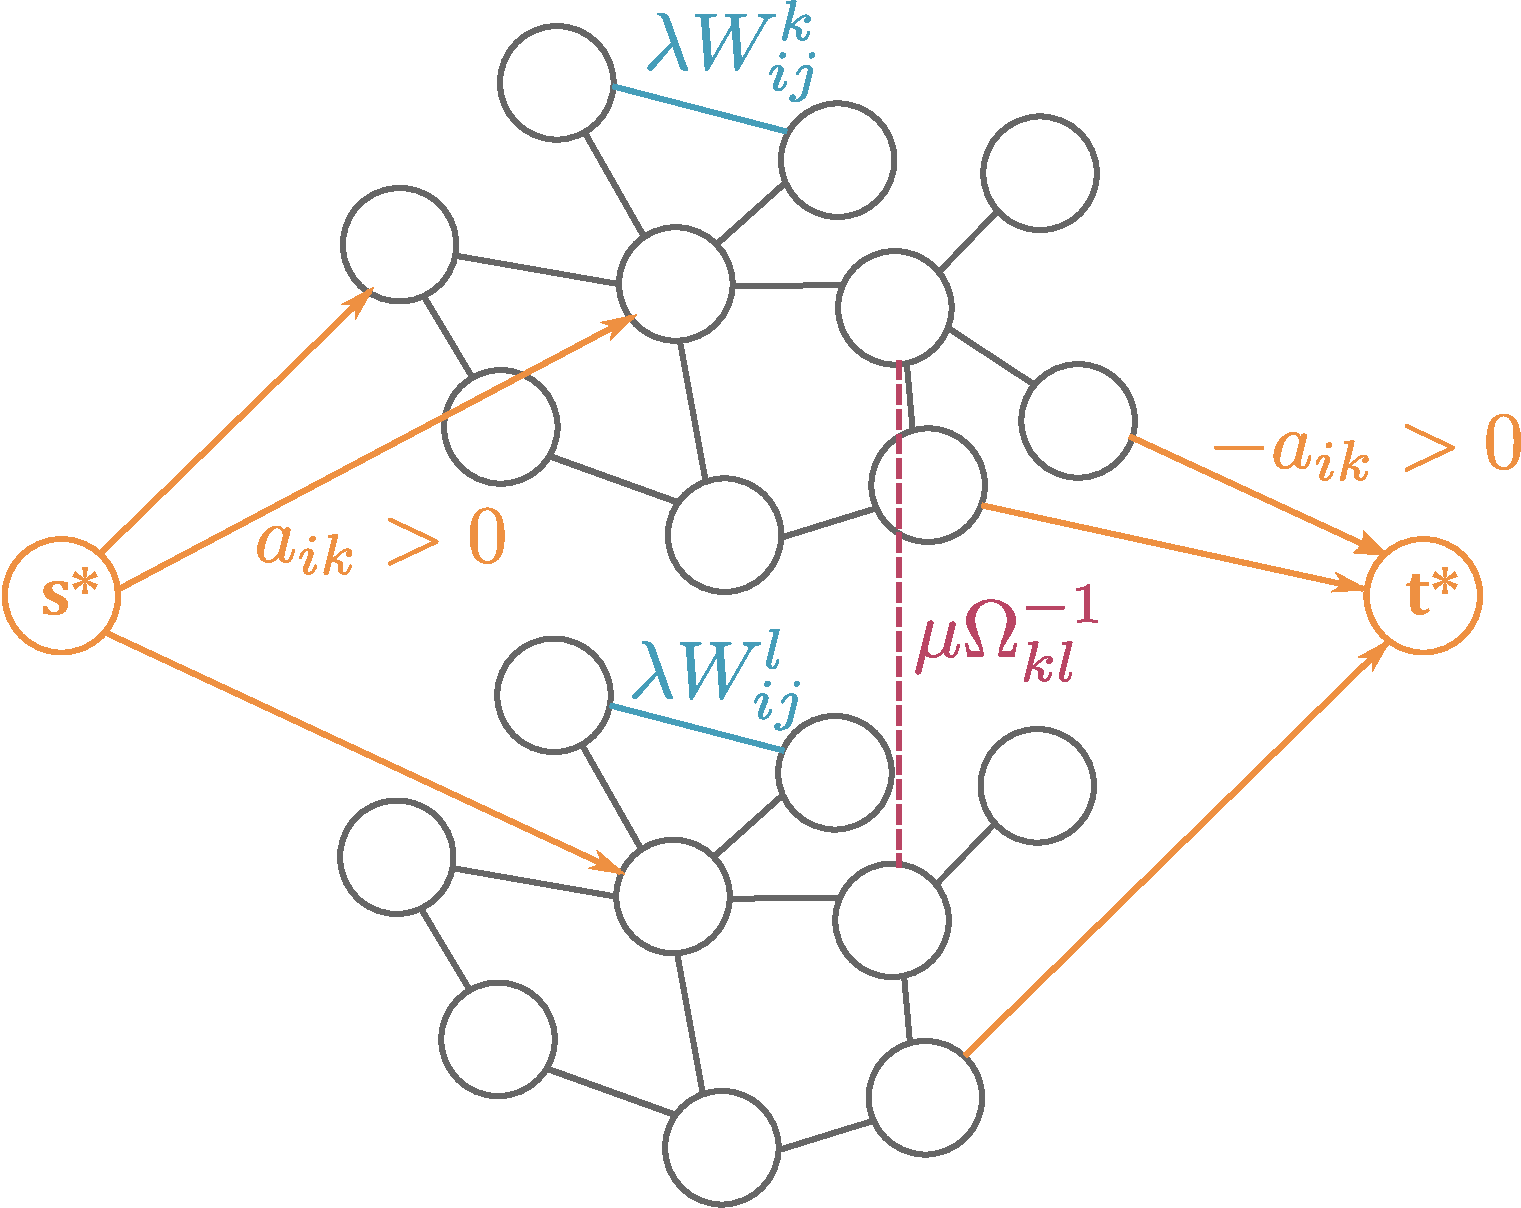
\includegraphics[width=0.5\textwidth]{figures/mincut_msfan}
  \caption{Finding the minimum cut of this super-network is equivalent to solving the multitask network-guided feature selection problem defined by Eq.~\ref{eq:msfan}.}
  \label{fig:mincut_msfan}
\end{figure}

\paragraph{Generality}
This formulation is equivalent to the two previous formulations:
\begin{itemize}
\item If $\mu=0$, then this is equivalent to formulating SConES (Eq.~\ref{eq:scones}) on each task independently.
\item If $\Omega^{-1}$ is defined by 
  \[
  \Omega_{kl}^{-1} = 
  \begin{cases}
     K - 1 + \epsilon & \mbox{ if } $k=l$ \\
     -1 & \mbox{otherwise},
  \end{cases}
  \]
 with $\epsilon > 0$, then this is equivalent to MultiSConES (where no covariance matrix is specified), 
with \[
\eta_{\mbox{multiscones}} = \eta + \mu \epsilon.
\]

Indeed, this yields $\Phi_k = \epsilon$, and Eq.~\ref{eq:msfan_mineq} then becomes
\[
  \argmin_{\sset_1, \ldots, \sset_K \subseteq \vset} \sum_{k=1}^K \left(
    \sum_{i \in \sset_k} - \left(c_i^k - \eta - \mu \epsilon \right) + 
    \sum_{i \in \sset_k} \sum_{j \notin \sset_k} \lambda W_{ij}^k \right) + 
  \sum_{k=1}^K \sum_{l=1}^K \left( \sum_{i \in \sset_k \setminus \sset_l} \mu \right).
\]

In this case, $\Omega$ is given by 
  \[
  \Omega_{kl} = 
  \begin{cases}
     \frac{1 + \epsilon}{\epsilon (K+\epsilon)} & \mbox{ if } $k=l$ \\
     \frac{1}{\epsilon (K+\epsilon)} & \mbox{otherwise}.
  \end{cases}
  \]
 $\Omega$ is close to a matrix of all ones, which is consistant with the idea that information should be shared across tasks, without accounting for task similarity.

% Indeed, for a given $(k, l)$, $|\sset_k \cap \sset_l| \Omega_{kl}^{-1}$ can be rewritten as :
% \[|\sset_k \cup \sset_l| \Omega_{kl}^{-1} - |\sset_k \Delta \sset_l| \Omega_{kl}^{-1}. \]
\end{itemize}


\section{Range of hyperparameters}

\subsection{Hyperparameters for MultiSConES}
\paragraph{Setting $\pmb{\eta}$} To avoid trivial solutions (in which either all features or no features are selected), one must ensure that not all nodes are connected to the source (resp. sink). This implies that some values of $(c_i^k - \eta)$ are positive and others are negative.\\

This implies $\max_{i. k} c_i^k - \eta > 0$ and $\min_{i. k} c_i^k - \eta < 0$. 

Setting $\eta_{\max} := \frac{\max_{i, k} c_i^k}{2}$ and $\eta_{\min} := 2 \min_{i, k} c_i^k$, we want values of $\eta$ to spread between these extrema.

We use 

\[\boxed{
\eta \in \left \{ {\eta_{\min} + \frac{t}{T} \left(\eta_{\max} - \eta_{\min} \right)    }   \right \}_{t = 0, \dots, (T-1)}}. 
\]

\paragraph{Setting $\pmb{\lambda}$} In order to make use of both the relevance scores and the network information, 
the values of $\lambda W_{ij}^k$ must be of similar magnitude to that of $|c_i^k - \eta|$. 
We take this to mean that $\lambda W_{ij}^k$ should take values spread around the median value of $|c_i^k - \eta|$, between its largest and its smallest values.\\

Denoting by $W_{\min}$ the smallest non-zero value of $W$ : 
$W_{\min} := \min_{i, j, k} \{ W_{ij}^k | W_{ij}^k \neq 0\}$,
we propose to consider 
\[
\lambda_{\max} := \frac{\max_{i,k} |c_i^k - \eta|}{W_{\min}}, 
\lambda_{\min} := \frac{\min_{i,k} |c_i^k - \eta|}{\max_{i,j,k}W_{ij}^k} \mbox{ and }
\lambda_{m} := \frac{\mbox{median}_{i, k} |c_i^k - \eta|}{\max_{i,j,k}W_{ij}^k}.
\]

 We then use 
\[\boxed{
\log_{10}(\lambda) \in \left \{ {\log_{10}(\lambda_{m}) - \frac{t}{(T+1)/2} 
 \left (\log_{10}(\lambda_{m}) - \log_{10}(\lambda_{\min}) \right)} \right \}_{t = 1, \dots, (T+1)/2}}
\]

 and

\[\boxed{
\log_{10}(\lambda) \in \left \{ {\log_{10}(\lambda_{m}) + \frac{t}{T/2} 
\left (\log_{10}(\lambda_{\max}) - \log_{10}(\lambda_{m}) \right)} \right \}_{t = 0, \dots, T/2}}.
\]


\paragraph{Setting $\pmb{\mu}$} Similarly, $\mu$ should take values of similar magnitude to that of $|c_i^k - \eta|$. We consider 
\[
\mu_{\max} := \max_{i,k} |c_i^k - \eta|,
\mu_{\min} := \min_{i,k} |c_i^k - \eta| \mbox{ and }
\mu_{m} := \mbox{median}_{i, k} |c_i^k - \eta|.
\]

 We then use 
\[\boxed{
\log_{10}(\mu) \in \left \{ {\log_{10}(\mu_{m}) - \frac{t}{(T+1)/2} 
 \left (\log_{10}(\mu_{m}) - \log_{10}(\mu_{\min}) \right)} \right \}_{t = 1, \dots, (T+1)/2}}
\]

 and

\[\boxed{
\log_{10}(\mu) \in \left \{ {\log_{10}(\mu_{m}) + \frac{t}{T/2} 
\left (\log_{10}(\mu_{\max}) - \log_{10}(\mu_{m}) \right)} \right \}_{t = 0, \dots, T/2}}.
\]



\subsection{Hyperparameters for multitask feature selection with a matrix of task covariance}
\paragraph{Setting $\pmb{\mu}$} To avoid trivial solutions (in which either all features or no features are selected), one must ensure that not all nodes are connected to the source (resp. sink). This implies that some values of $a_i^k$ are positive and others are negative.\\

By definition, $a_i^k = c_i^k - \mu \phi_k - \eta$. As
\[
\min_{i, k} c_i^k - \mu \max_k \phi_k - \eta \leq 
  a_i^k   \leq \max_{i, k} c_i^k - \mu \min_k \phi_k - \eta,
\]
this implies that $(\min_{i, k} c_i^k - \mu \max_k \phi_k - \eta) < 0$ and
$(\max_{i, k} c_i^k - \mu \min_k \phi_k - \eta) > 0$.\\

Hence, if $\mu$ is given, $\eta$ must be chosen smaller than 
$( \max_{i, k} c_i^k - \mu \min_k \phi_k )$.\\

Because we want $\eta$ to be strictly positive (to enforce sparsity), this in turn implies that\\ $\max_{i, k} c_i^k - \mu \min_k \phi_k > 0$. If $\min_k \phi_k < 0$, this is guaranteed. Otherwise our first condition is:
\[ \mu < \frac{\max_{i, k} c_i^k}{\min_k \phi_k}.\]

We hence set $\mu_{\max} := \frac{\max_{i, k} c_i^k}{|\min_k \phi_k|}$.\\

In our experiments, we use 
\[ \boxed{
\mu \in \left\{ \frac{\mu_{\max}}{2^{t+1}} \right \}_{t = 0, \dots, (T-1)}}.
\]

\paragraph{Setting $\pmb{\eta}$} $\mu$ being set, we can compute 
$\eta_{\max} := \frac{1}{2} (\max_{i, k} c_i^k - \mu \min_k \phi_k)$ and 
$\eta_{\min} := 2 (\min_{i, k} c_i^k - \mu \max_k \phi_k)$.

%  and use $\eta \in 
% \left \{ \frac{\eta_{\max}}{10 \times 2^t} \right \}_{t = 0, \dots, (T-1)}$.\\

If $\eta_{\min} > 0$, we then want values of $\eta$ to spread between these extrema.
We use 
\[\boxed{
\log_{10}(\eta) \in \left \{ {\log_{10}(\eta_{\min}) + \frac{t}{T} \left(\log_{10} \left(\eta_{\max}\right) - \log_{10}(\eta_{\min}) \right)    }   \right \}_{t = 0, \dots, (T-1)}}. 
\]

Else, we simply use 
\[ \boxed{
\eta \in \left \{ \frac{\eta_{\max}}{2^{t+1}} \right \}_{t = 0, \dots, (T-1)}}.
\]

\paragraph{Setting $\pmb{\lambda}$} In order to make use of both the relevance scores and the network information, 
the values of $\lambda W_{ij}^k$ must be of similar magnitude to that of $|a_i^k|$. 
We take this to mean that $\lambda W_{ij}^k$ should take values spread around the median value of $|a_i^k|$,
between its largest and its smallest values.\\

Denoting by $W_{\min}$ the smallest non-zero value of $W$ : 
$W_{\min} := \min_{i, j, k} \{ W_{ij}^k | W_{ij}^k \neq 0\}$,
we propose to consider 
\[
\lambda_{\max} := \frac{\max_{i,k} |a_i^k|}{W_{\min}}, 
\lambda_{\min} := \frac{\min_{i,k} |a_i^k|}{\max_{i,j,k}W_{ij}^k} \mbox{ and }
\lambda_{m} := \frac{\mbox{median}_{i, k} |a_i^k|}{\max_{i,j,k}W_{ij}^k}.
\]

 We then use 
\[\boxed{
\log_{10}(\lambda) \in \left \{ {\log_{10}(\lambda_{m}) - \frac{t}{(T+1)/2} 
 \left (\log_{10}(\lambda_{m}) - \log_{10}(\lambda_{\min}) \right)} \right \}_{t = 1, \dots, (T+1)/2}}
\]

 and

\[\boxed{
\log_{10}(\lambda) \in \left \{ {\log_{10}(\lambda_{m}) + \frac{t}{T/2} 
\left (\log_{10}(\lambda_{\max}) - \log_{10}(\lambda_{m}) \right)} \right \}_{t = 0, \dots, T/2}}.
\]



\paragraph{Remark.} In our experiments, we use a random sample of $50\%$ of the values of $c_i^k$ to set the ranges of values for the hyperparameters $\mu$, $\eta$ and $\lambda$ before starting.


\bibliographystyle{plain}
\bibliography{references}
\end{document}
